\subsection{Imaging in LM and N}
\label{ssec:overview_lm_imaging}

\textbf{Note: The pipeline layout has been modified compared to the
  PDR design in order to achieve better modularity. Basic reduction
  and background subtraction have been split into two recipes that now
  are applied to both standard and science data. Integration of \ac{HCI}
  into this workflow requires more work: \ac{HCI} images will be treated
  the same way at least through basic reduction, possibly through
  background subtraction. \ac{ADI} combination may require a separate
  recipe, at least for some \ac{HCI} configurations.}

The purpose of the pipeline is to correct or remove contributions from
the instrument, telescope, and atmosphere and produce science-grade
data products.  In the case of the METIS imaging modes the main
contributions to correct or remove are dark current, flatfield, bad
pixels, and, most importantly, thermal background emission from the
sky and the telescope. Further effects include persistence,
cross-talk, geometric distortions, etc. The final product of the
imaging pipeline is one or more flux-calibrated image(s) in units of
photons/s/pixel. Several images can be stacked into a single possibly
mosaiced image.

Due to the differences in characteristics between the HAWAII2RG
detector used for imaging in the L and M bands and the GeoSnap
detector used for the N band, the operational concept for the two
imager subsystems are quite different. This induces differences in the
way the data have to be reduced.

The GeoSnap detector has more stable gain than AQUARIUS detector,
which was still in the baseline at PDR.  Chopping is still necessary,
albeit at a lower frequency of a few Hz, and the standard chop/nod
technique will be employed for background subtraction.  As the dark
signal is automatically removed when the exposures from the different
chop and nod positions are combined no master dark is required for the
reduction of science data. Flat fielding may be possible, pending
further investigation of the detector stability

Observations and reduction of LM band data with the HAWAII2RG detector
can proceed as in the near infrared. After dark subtraction and
flat-fielding, the background is estimated from a series of dithered
science exposures or from exposures on a nearby blank patch of sky.

The association maps for the current designs of the imaging pipelines
in~LM and~N are shown in Figs.~\ref{fig:IMG_LM_Assomap}
and~\ref{fig:IMG_N_Assomap}, respectively.

\TODO{For \ac{HCI} data, \ac{ADI} may need to be part of reduction recipe if
  individual background subtracted images are the goal?}


\begin{sidewaysfigure}
  \centering
  \centerline{\resizebox{\textwidth}{!}{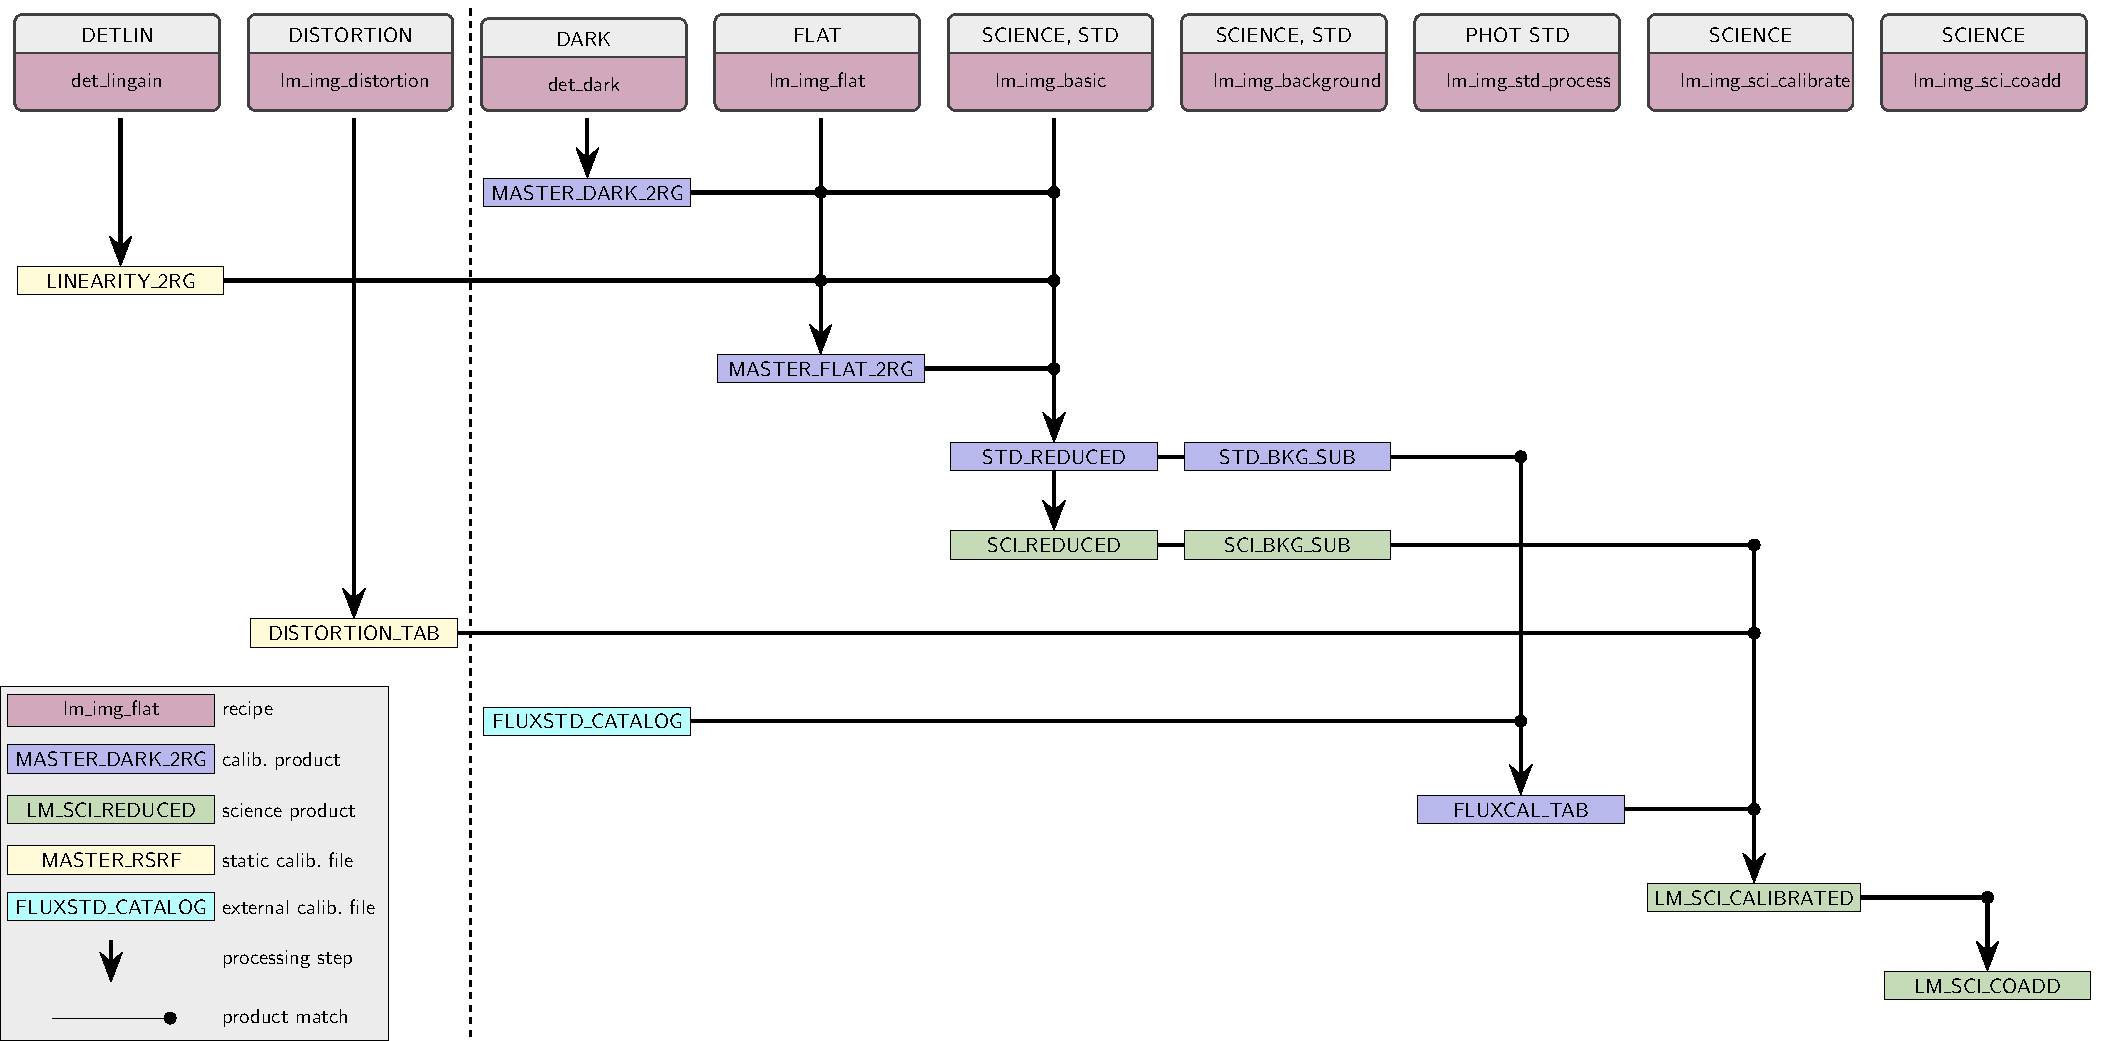
\includegraphics{IMG_LM_assomap_tikz}}}
  \caption[Reduction cascade and association map for imaing in L and
  M]{Association map for imaging in the LM band. The figure shows only
    the primary product created from each recipe; for a full list of
    products refer to the recipe descriptions in
    Sect.~\ref{ssec:recipes_img_lm}. The dashed line separates
    calibration tasks that are done at AIT or infrequently during
    operations (left) from daily tasks (right). The prefix ``\REC{metis_}'' has been
    omitted from the recipe names to improve clarity. The product
    names omit ``\PROD{LM_}''.}
  \label{fig:IMG_LM_Assomap}
\end{sidewaysfigure}


\begin{sidewaysfigure}
  \centering
  \centerline{%
    \resizebox{\textwidth}{!}{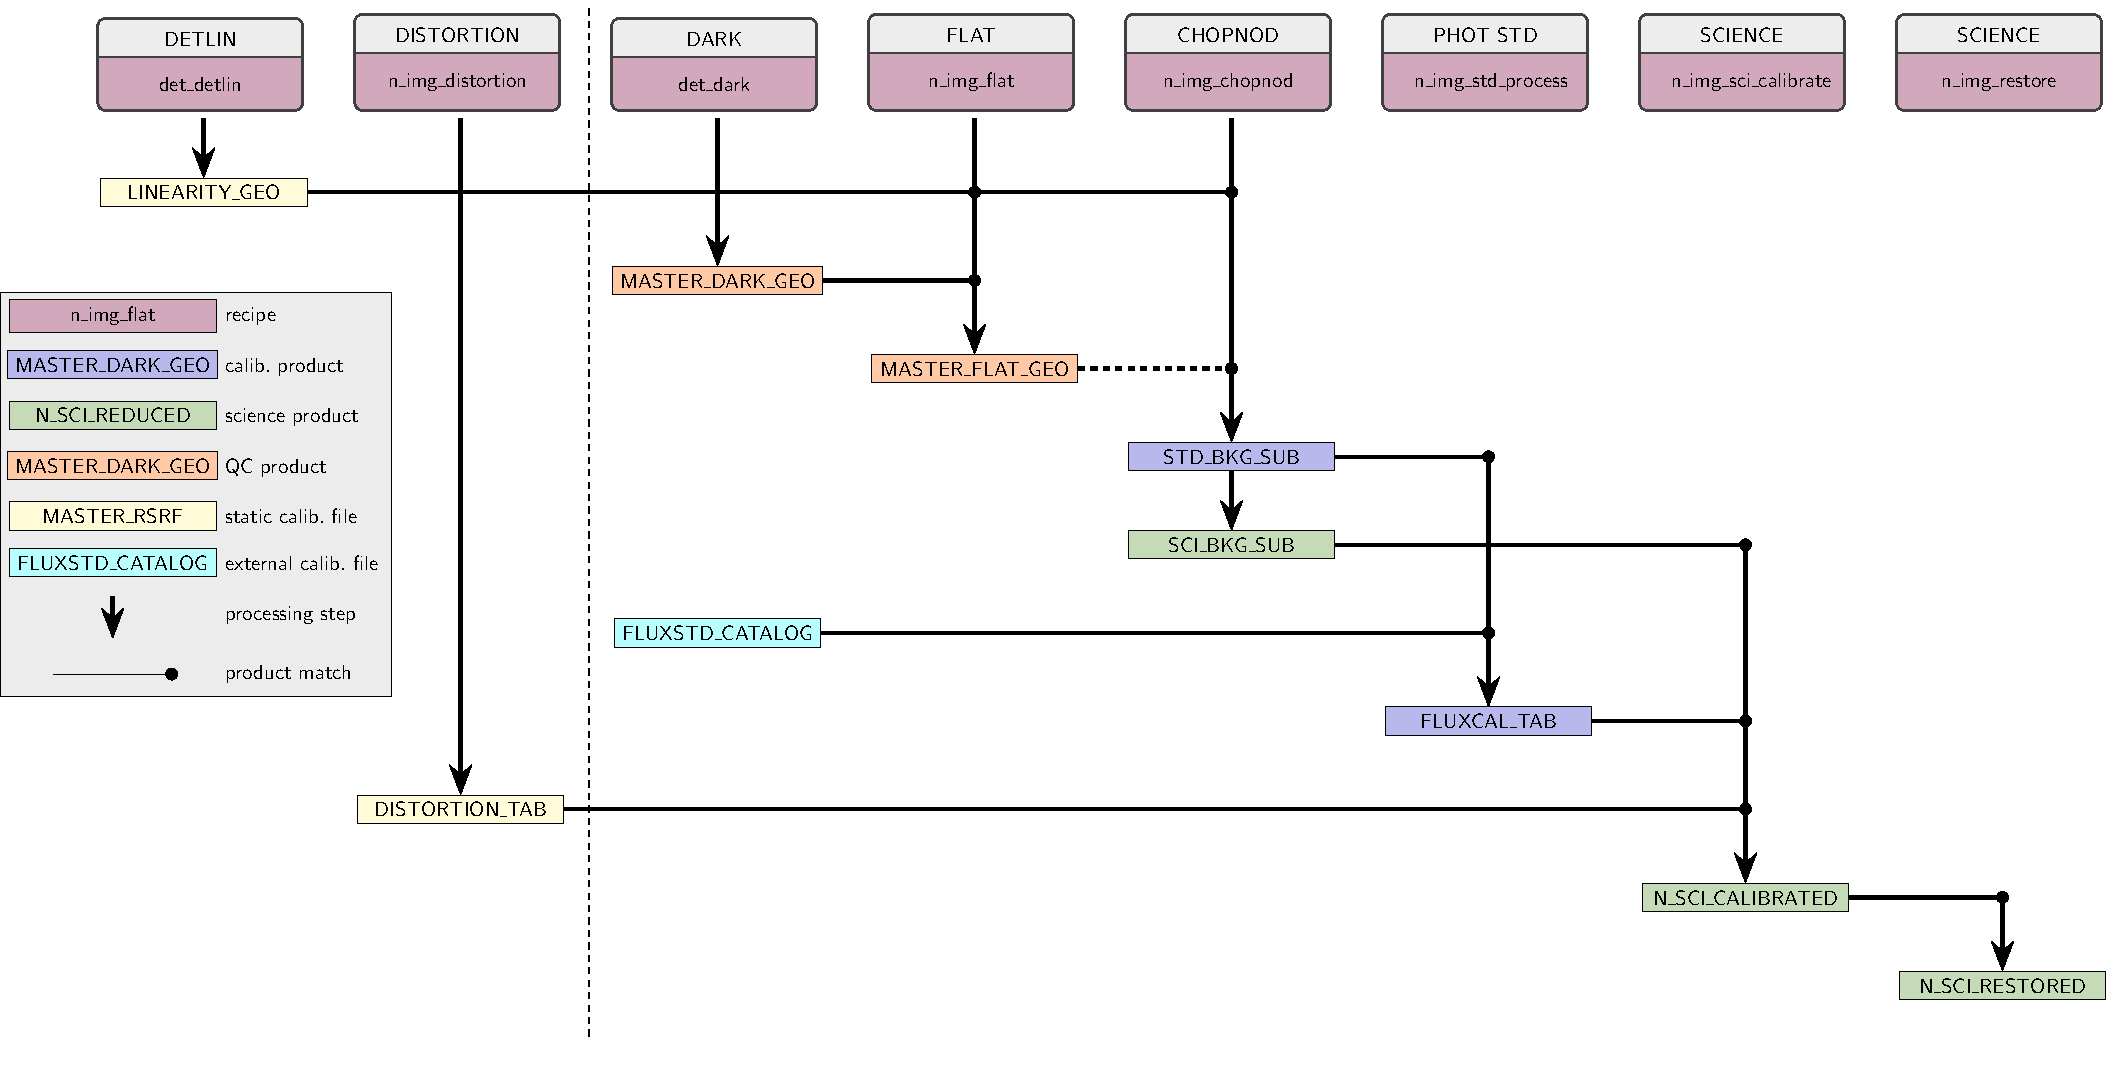
\includegraphics{IMG_N_assomap_tikz}}
  }
  \caption[Reduction cascade and association map for imaing in N]{%
    Association map for imaging in the N band. The figure shows
    only the primary product created from each recipe; for a full
    list of products refer to the recipe descriptions in
    Sect.~\ref{ssec:recipes_img_n}. The dashed line separates
    calibration tasks that are done at AIT or infrequently during
    operations (left) from daily tasks (right). The prefix ``\REC{metis_}'' has
    been omitted from the recipe names to improve clarity. The
    product names omit ``\PROD{N_}''.}
  \label{fig:IMG_N_Assomap}
\end{sidewaysfigure}

%%%%%%%%%%%%%%%%%%%%%%%%%%%%%%%%%%%%%%%%%%%%%%%%%%%%%%
%%% Local Variables:
%%% TeX-master: "METIS_DRLD"
%%% End:
